
First, Section~\ref{sec:estep_sleep_compare} motivates the wake-sleep approach by comparing variational posteriors obtained by optimizing the ELBO against those obtained by optimizing the sleep objective. 
Then, StarNet is tested on blended simulated stars in Section~\ref{sec:deblending_test}. 
Finally, in Section~\ref{sec:results_on_m2} we employ StarNet to catalog the SDSS image of the M2 globular cluster and show that StarNet produces higher quality detections compared with prior work on probabilistic cataloging. 


\subsection{ELBO versus sleep objective}
\label{sec:estep_sleep_compare}

In this subsection, we compare the resulting variational posteriors obtained by optimizing the sleep objective~\eqref{eq:sleep_obj} 
against those obtained by optimizing the ELBO~\eqref{eq:elbo}.
This simple example demonstrates that there exist shallow optima in the ELBO where the variational posterior on locations does not concentrate around the true locations.
On this example, fitting the variational posterior using the sleep phase is able to avoid shallow optima. 
Because the data were simulated with known PSF and background, the wake-phase is not needed. 

The simulated $20\times20$ single-band image $x_{test}$ is shown in Figure~\ref{fig:toy_example}.
The image has four stars, each with the same flux. It is partitioned into four $10\times 10$ tiles, which are the inputs to the neural network. 
The image was fixed for this experiment. 

\begin{figure}[!h]
    \centering
    \vspace{-1em}
    \includegraphics[width = 0.3\textwidth]{figures/vi_sleep_ex_figure.png}
    \vspace{-1.7em}
    \caption{Our $20\times 20$ pixel test image with four stars, partitioned into $10\times 10$ tiles. }
    \label{fig:toy_example}
\end{figure}

In our generative model, we set the prior on the number of stars $N$ to have mean $\mu = 4$ and the prior on flux to have power law slope $\alpha = 0.5$. 
With these prior parameters, we compare directly optimizing the ELBO on the test image, 
\begin{align}
\mathcal{L}_{elbo}(\eta; x_{test}) = \Expect_{q_{\eta}(z | x_{test})}\Big[\log p(x_{test}, z) - \log q_{\eta}(z | x_{test})\Big],
\label{eq:elbo_on_test}
\end{align}
against optimizing the sleep objective $\mathcal{L}_{sleep}(\eta)$ in~\eqref{eq:sleep_obj}. Note that optimizing the sleep objective does not depend on $x_{test}$: the sleep phase only requires sampling catalogs from the aforementioned prior and the simulating images given the catalog. 

Figure~\ref{fig:optim_path} charts the ELBO~\eqref{eq:elbo_on_test} as the optimization proceeds.
In the first approach (Figure~\ref{fig:optim_path}a), the ELBO was optimized with stochastic gradient descent and the REINFORCE estimator.
This optimization did not converge, likely due to the high variance of the REINFORCE estimator. 
For a lower variance gradient estimator, the second approach (Figure~\ref{fig:optim_path}b) employed the reparameterized gradient.  To employ this gradient estimator, we analytically integrated the ELBO with respect to the number of stars $N$ to remove the discrete random variable. 
See Appendix~\ref{sec:reparam_details} for details about the gradient estimators. 
The lower variance of the reparameterized gradients allowed the optimization to converge to stationary points. 
However, depending on the initialization, the variational distribution converged to points where the ELBO is non-optimal (e.g. restarts 3 and 6). 

In contrast, Figure~\ref{fig:optim_path}c shows the ELBO as the sleep phase proceeds. 
While the sleep phase does not directly optimize the ELBO, the ELBO increases nonetheless as the variational posterior approaches the true posterior in $\textrm{KL}$. 
Optimizing the sleep objective consistently converged to a similar ELBO across all restarts, and appeared to avoid the shallow local optimum found in Figure~\ref{fig:optim_path}b.

The bottom row of Figure~\ref{fig:optim_path} displays the estimated locations, given by the mode of the fitted variational distribution. 
The bottom left shows these locations after getting stuck in a local minimum. 
In the tile with two stars, both estimated locations were placed on one star. 
For correct detections, one of the locations should be placed on the second star. 
However, to move one location to the second star, the optimization path must traverse a region where the log-likelihood is lower than the current configuration. 
The displayed configuration is a local optima where the gradient with respect to its locations is approximately zero.
In contrast, the sleep phase optimization consistently placed its mode around the four true stars. 
An example of correct detections after sleep phase optimization is shown in the bottom right of~Figure~\ref{fig:optim_path}.

\begin{figure}[!htb]
    \centering
    \begin{subfigure}[t]{0.9\textwidth}
    \centering
    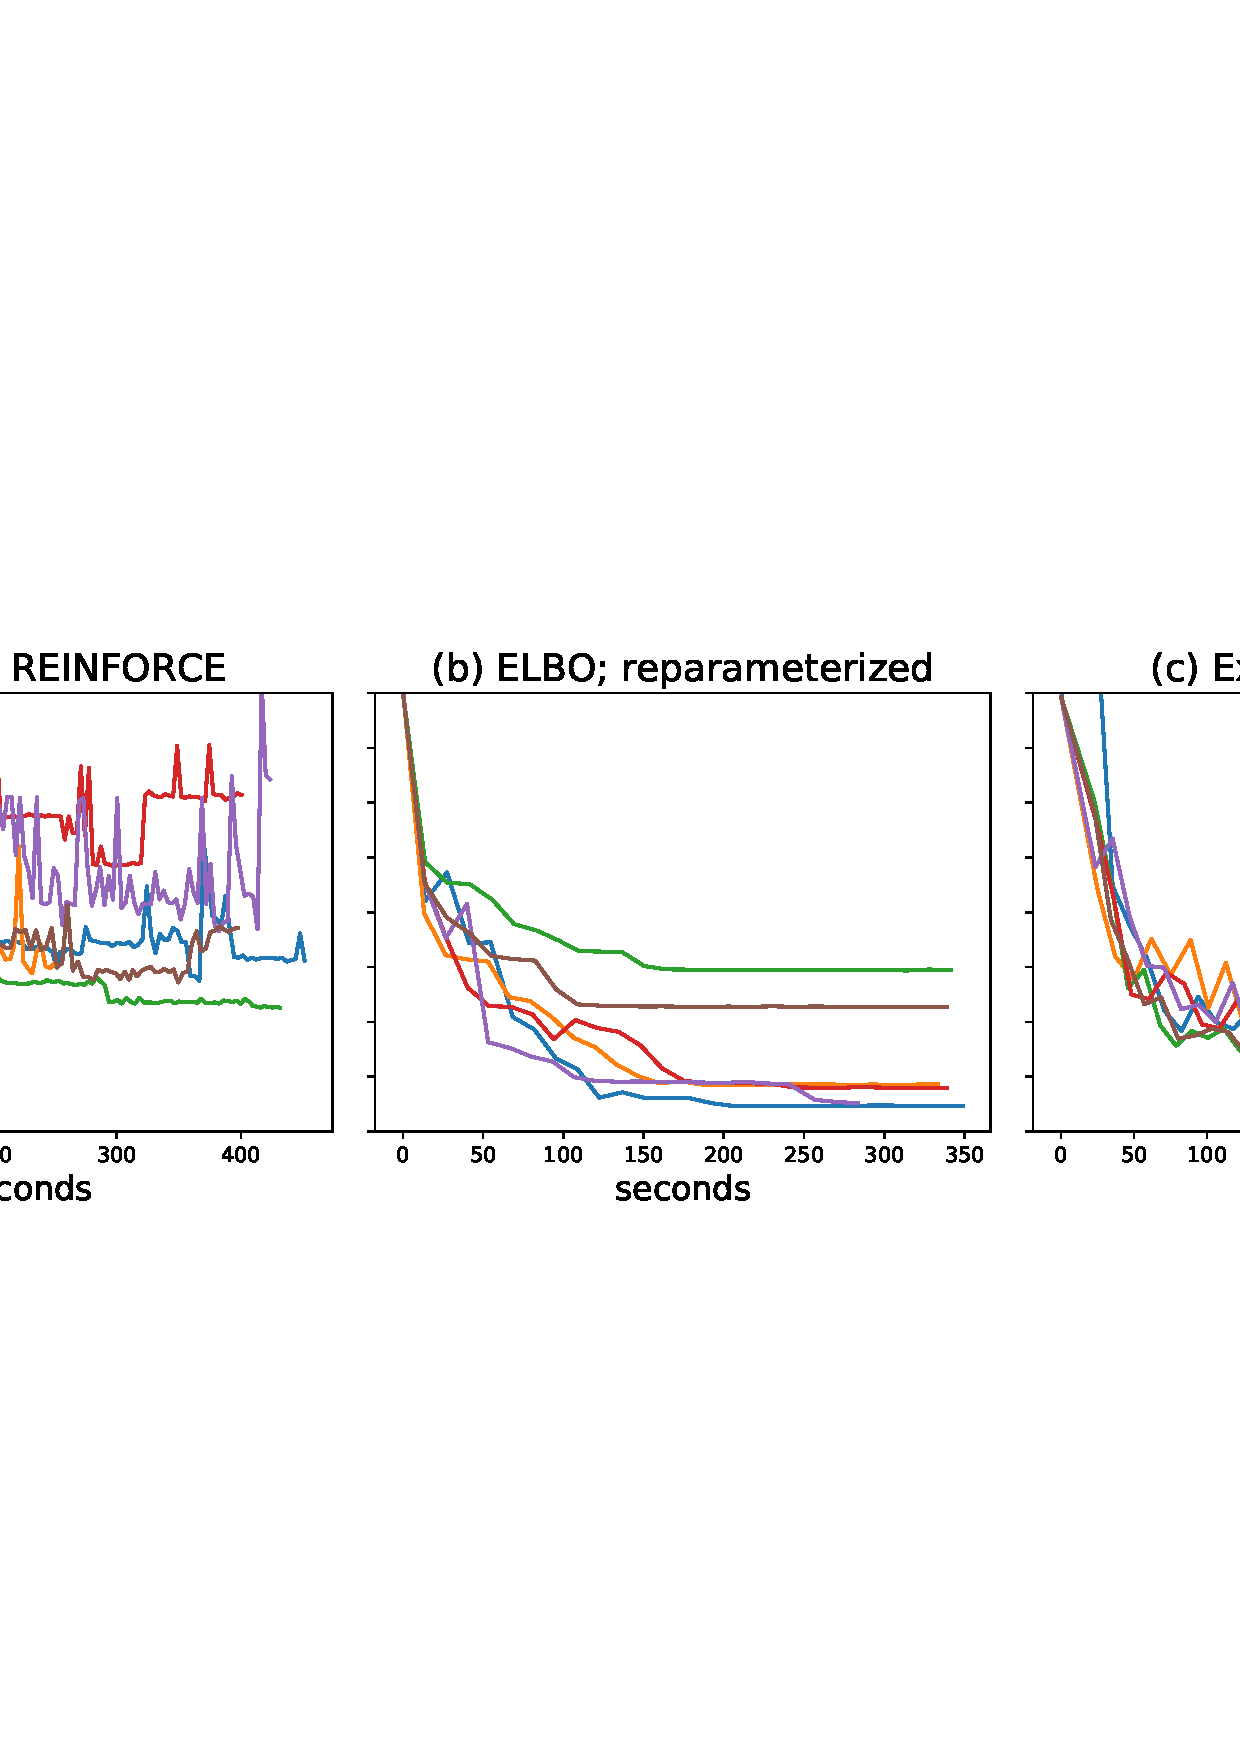
\includegraphics[width=\textwidth]{figures/optim_path_compare.png}
    \end{subfigure}
    \begin{subfigure}[t]{\textwidth}
    \centering
    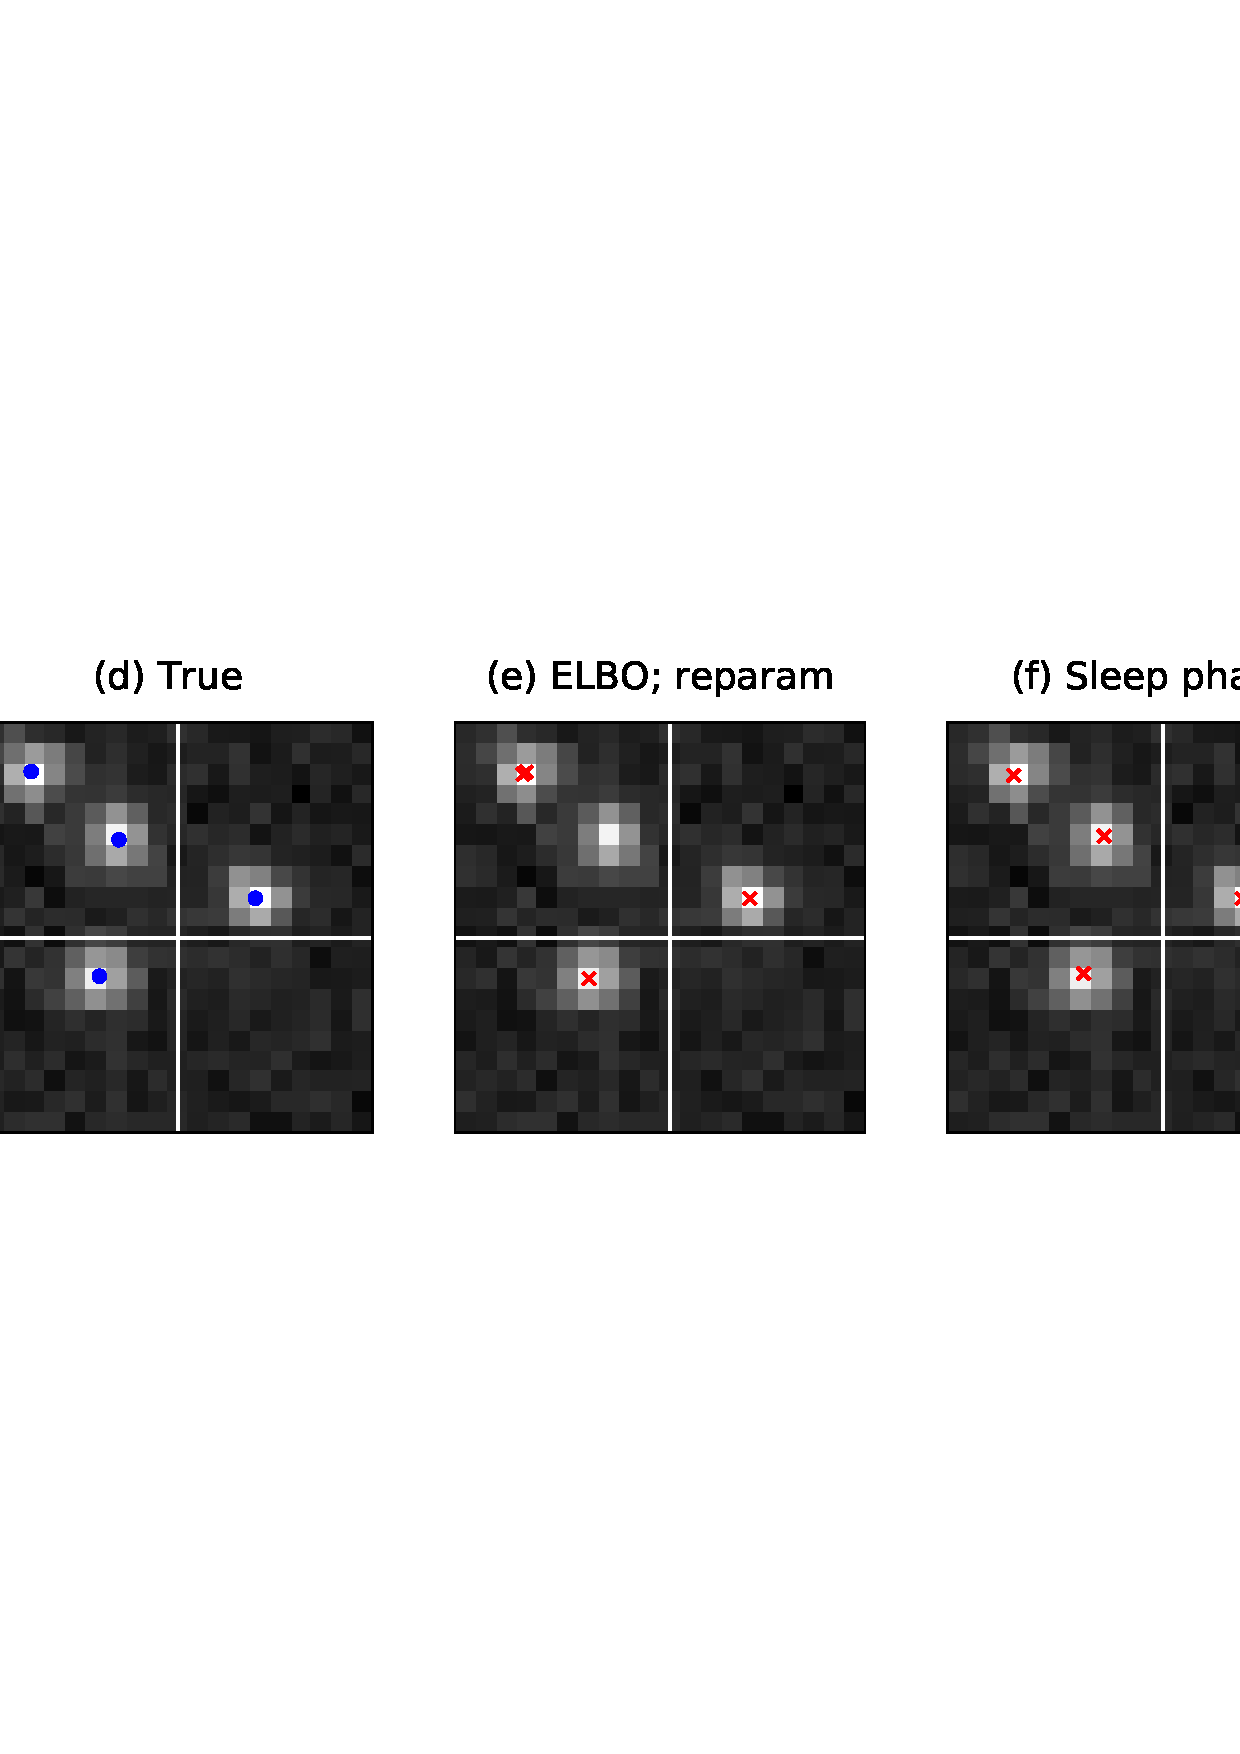
\includegraphics[width=0.55\textwidth]{figures/optim_path_detect_compare.png}
    \end{subfigure}
    \vspace{-3em}
    \caption{(Top row) The ELBO as the optimization progresses 
    for six random restarts. 
    The bold pink line in all plots is the sleep phase ELBO path, averaged over six restarts. 
    (Bottom row) Estimated locations from two variational posteriors shown in red. On the left, an instance where optimizing the ELBO using the reparameterized gradient landed in a local optimum.
    On the right, an example of detections under 
    sleep-optimized variational posterior. }
    \label{fig:optim_path}
\end{figure}

Figure~\ref{fig:gradzero_cartoon} shows schematic of this general phenomenon. When the estimated location is far from the true location, the gradient of the ELBO with respect to location vanishes. Because the PSF is nearly zero everywhere except for a few pixels around each location, a small shift in location does not significantly change the likelihood unless the estimated location is within a ``PSF radius" of the true location. On the other hand, the sleep phase objective is quadratic in the estimated location -- see~\eqref{eq:gaussian_sleep_loss}. Thus, the further the estimated location from the true location, the larger the gradient. The gradient does not vanish in the sleep objective. 

\begin{figure}[!htb]
    \centering
    \begin{subfigure}[t]{0.8\textwidth}
    \centering
    \includegraphics[width=\textwidth]{figures/gradzero_cartoon.png}
    \end{subfigure}
    \begin{subfigure}[t]{\textwidth}
    \centering
    \includegraphics[width=0.55\textwidth]{figures/gradzero_cartoon2.png}
    \end{subfigure}
    \vspace{-3em}
    \caption{An illustration of vanishing gradients. Because the estimated star is far from the true star, the log-likelihood (and relatedly the ELBO) does not change for any location in an $\epsilon$-ball of the estimated location. 
    For large delta, the gradient of the ELBO with respect to locations is zero. In contrast, the sleep objective is quadratic in the estimated location, and the gradient does not vanish. }
    \label{fig:gradzero_cartoon}
\end{figure}

Also note that low-variance gradients of the ELBO were constructed by analytically integrating $N$ in the objective, so the reparameterization trick could be applied. 
In this example, $N_{max} = 2$ so the neural network infers either 0, 1, or 2 stars on each tile. 
Since the variational distribution factorizes over the four tiles, integrating $N$ is a summation of $3^4 = 81$ terms.
On larger images with more tiles, analytically integrating $N$ would be computationally infeasible, and REINFORCE gradients would be required. 

To illustrate on a larger example, Figure~\ref{fig:sim_data100x100} displays our results on a simulated $100\times 100$ image with fifty stars. The tiles again consisted of $10\times 10$ pixels. Optimizing the sleep phase objective resulted in near perfect in estimation of locations; optimizing the ELBO appears to be hindered by regions with little gradient information and is slow to converge. 

\begin{figure}[!htb]
    \centering
    \begin{subfigure}[!t]{0.4\textwidth}
    \centering
    \includegraphics[width=\textwidth]{figures/optim_path_compare_100x100.png}
    \end{subfigure}
    \begin{subfigure}[!t]{0.59\textwidth}
    \centering
    \includegraphics[width=\textwidth]{figures/optim_path_detect_compare_100x100.png}
    \end{subfigure}
    \caption{(Left) The negative conditional log-likelihoood $p(x|\hat z)$, where $\hat z$ is the mode of the variational posterior. (Right) Detections on a $100\times 100$ image, with true locations in blue, and estimated locations in red. }
    \label{fig:sim_data100x100}
\end{figure}
